\documentclass[11pt,a4paper]{article}

% Manual de usuario de MSX StepUp HybridHLE.
% Compilar desde esta carpeta con: make
\usepackage[utf8]{inputenc}
\usepackage[T1]{fontenc}
\usepackage[spanish,es-nodecimaldot]{babel}
\usepackage[a4paper,margin=22mm,headheight=15pt]{geometry}
\usepackage{graphicx}
\usepackage{array}
\usepackage{tabularx}
\usepackage{booktabs}
\usepackage{xcolor}
\usepackage{hyperref}
\usepackage{fancyhdr}
\usepackage{enumitem}

\definecolor{msxblue}{HTML}{087EB8}
\definecolor{stepred}{HTML}{EF3B45}
\definecolor{ink}{HTML}{172033}
\definecolor{softblue}{HTML}{EAF6FB}
\definecolor{softgray}{HTML}{F2F4F7}

\hypersetup{
  colorlinks=true,
  linkcolor=msxblue,
  urlcolor=msxblue,
  pdftitle={Manual de usuario de MSX StepUp HybridHLE},
  pdfauthor={DiHalt (Fernando García y Clemente Tiñena)}
}

\graphicspath{{../../assets/graphics/}}
\setlength{\parindent}{0pt}
\setlength{\parskip}{0.65em}
\setlist{itemsep=0.25em,topsep=0.35em}
\renewcommand{\arraystretch}{1.25}

\pagestyle{fancy}
\fancyhf{}
\fancyhead[L]{\textcolor{msxblue}{MSX StepUp HybridHLE}}
\fancyhead[R]{Manual de usuario}
\fancyfoot[C]{\thepage}
\renewcommand{\headrulewidth}{0.4pt}

\newcommand{\tecla}[1]{%
  \begingroup
  \setlength{\fboxsep}{3pt}%
  \colorbox{softgray}{\texttt{#1}}%
  \endgroup
}

\newcommand{\aviso}[2]{%
  \begin{center}
  \fcolorbox{#1}{softblue}{%
    \begin{minipage}{0.91\textwidth}
      #2
    \end{minipage}}
  \end{center}
}

\begin{document}

\begin{titlepage}
  \thispagestyle{empty}
  \centering
  \vspace*{8mm}
  
\includegraphics[width=0.76\textwidth]{stepup_logo.png}

  \vspace{8mm}
  {\Huge\bfseries\color{ink} Manual de usuario\par}
  \vspace{2mm}
  {\Large El juego original de MSX, envuelto en una capa moderna\par}

  \vfill
  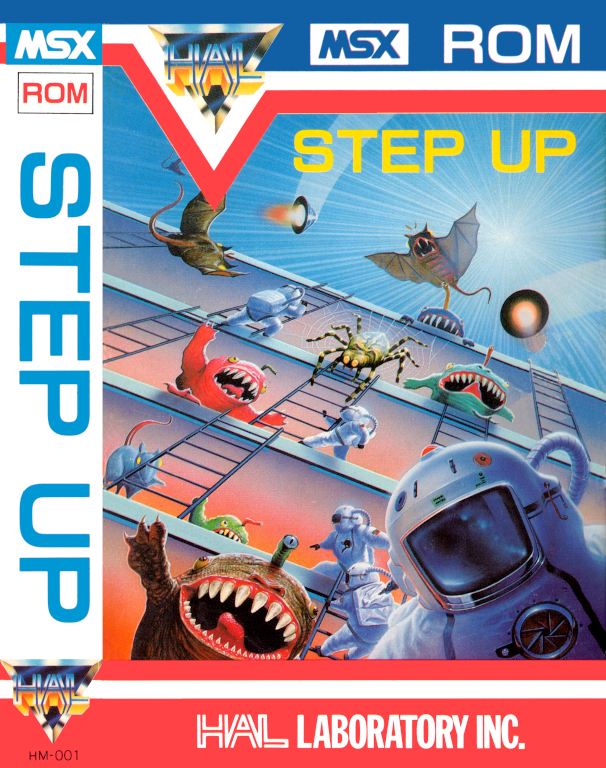
\includegraphics[height=0.59\textheight,keepaspectratio]{intro.png}
  \vfill

  {\large Versión 1.0 --- agosto de 2026\par}
  \vspace{2mm}
  {\small DiHalt --- Fernando García y Clemente Tiñena\par}
\end{titlepage}

\tableofcontents
\newpage

\section{Bienvenido a Step Up}

\textit{Step Up} es un juego de acción y plataformas publicado originalmente
para MSX en 1983 y desarrollado por Takara y Marvel Soft. Encarnas a un
astronauta solitario atrapado en un planeta hostil. Su única posibilidad de
regresar a casa es subir hasta la azotea y alcanzar la nave espacial.

\textbf{MSX StepUp HybridHLE conserva el programa original del cartucho.} No
es un remake que imite sus reglas: las instrucciones originales para el
microprocesador Z80 siguen decidiendo el movimiento, las colisiones, los
enemigos, la puntuación, las vidas y el avance entre fases. Godot actúa como
una capa exterior moderna que permite ejecutar y presentar ese programa en
Windows, Linux, macOS y Android.

\aviso{stepred}{\textbf{Importante.} El cartucho original no se distribuye con
el proyecto. Para jugar necesitas un volcado obtenido legalmente de tu propio
cartucho de \textit{Step Up}.}

\section{Puesta en marcha}

\subsection{Primera ejecución}

\begin{enumerate}
  \item Abre \textbf{MSX StepUp HybridHLE}.
  \item Cuando aparezca la pantalla de configuración, pulsa
        \textbf{Select Step Up ROM}.
  \item Selecciona el archivo \texttt{.rom} de tu cartucho. Si se encuentra
        dentro de un ZIP, extráelo antes.
  \item El programa reconocerá volcados de 8, 16 o 32 KiB, extraerá el banco
        válido de 8 KiB y guardará una copia privada para las siguientes
        ejecuciones.
\end{enumerate}

En ordenadores de escritorio también puedes crear una carpeta
\texttt{roms} junto al ejecutable y guardar el archivo como
\texttt{roms/stepup.rom}. En macOS, la carpeta debe estar junto al paquete
\texttt{.app}, no dentro de él.

\subsection{Comenzar la partida}

Tras cargar el juego aparece una ilustración inicial durante unos segundos.
Pulsa \tecla{Espacio} ---o \textbf{ACTION} en Android--- para omitirla. En la
pantalla del título, usa igualmente el botón de acción para iniciar la partida
cuando el juego lo solicite.

\section{Objetivo del juego}

El edificio está formado por diez plantas, señaladas de F1 a F10 y comunicadas
por escaleras azules. Debes conducir al astronauta desde la zona inferior
hasta la azotea, evitando las criaturas y obstáculos que recorren cada piso.

Cuando alcances el tejado aparecerá una pequeña nave. \textbf{No basta con
llegar arriba: hay que saltar dentro antes de que se aleje.} Si lo consigues,
pasarás a la siguiente fase; si tardas demasiado, quedarás expuesto a los
enemigos de la azotea.

\subsection{Peligros}

Cada amenaza se comporta de forma distinta. Entre ellas encontrarás:

\begin{itemize}
  \item ratones o ratas que corren por las plataformas;
  \item murciélagos que vuelan verticalmente;
  \item monstruos que recorren escaleras y pisos;
  \item arañas que aparecen periódicamente desde sus telarañas;
  \item obstáculos móviles, como la viga roja.
\end{itemize}

El contacto puede hacer caer al astronauta hasta el suelo y cuesta una vida.
Después de perderla, vuelves a comenzar desde la parte inferior. La partida
empieza con tres vidas y concede una vida adicional cada 10.000 puntos.

\subsection{Barrera de energía}

El astronauta dispone de una protección temporal. Cuando está activa, el
personaje se vuelve rojo y consume parte del indicador de energía situado en
la parte inferior de la pantalla. La reserva se repone al comenzar una nueva
vida o una nueva fase; si se agota, el personaje queda derrotado.

Las fases posteriores mantienen el objetivo, pero aumentan la presión y la
cantidad de peligros; por ejemplo, aparecen más telarañas.

\section{Controles}

\begin{center}
\begin{tabularx}{\textwidth}{>{\bfseries}p{0.28\textwidth}XX}
\toprule
Acción & Ordenador & Android \\
\midrule
Caminar a izquierda o derecha & \tecla{$\leftarrow$} / \tecla{$\rightarrow$} & LEFT / RIGHT \\
Subir o bajar por una escalera & \tecla{$\uparrow$} / \tecla{$\downarrow$} & UP / DOWN \\
Saltar o realizar una acción & \tecla{Espacio} & ACTION \\
Omitir la ilustración inicial & \tecla{Espacio} & ACTION \\
\bottomrule
\end{tabularx}
\end{center}

En Android los cinco botones aparecen superpuestos en la pantalla. Las cuatro
direcciones están a la izquierda y \textbf{ACTION} a la derecha.

\subsection{Consejos de juego}

\begin{itemize}
  \item Observa primero la ruta y el ritmo de cada enemigo.
  \item Espera un hueco seguro antes de entrar en una escalera: mientras
        subes o bajas tienes menos opciones para esquivar.
  \item Reserva la barrera de energía para cruces difíciles.
  \item Al llegar al tejado, colócate para saltar a la nave sin demora.
  \item No te precipites. \textit{Step Up} premia la memoria y el ritmo más
        que la velocidad constante.
\end{itemize}

\section{Qué significa Hybrid HLE}

\textbf{Hybrid HLE} significa, en este proyecto, que se combina emulación de
bajo nivel para la CPU con sustituciones de alto nivel para servicios concretos
del MSX.

\begin{center}
\setlength{\fboxsep}{8pt}
\fcolorbox{msxblue}{softblue}{%
\begin{minipage}{0.88\textwidth}
\centering
Teclado o pantalla táctil
\(\longrightarrow\) matriz de teclado MSX
\(\longrightarrow\) código original Z80\\[3pt]
\(\longrightarrow\) memoria y VRAM
\(\longrightarrow\) imagen y sonido presentados por Godot
\end{minipage}}
\end{center}

La extensión nativa del proyecto emula el microprocesador Z80 y ejecuta las
instrucciones del cartucho. Al iniciar la partida se construye el espacio de
memoria de 64 KiB que ve esa CPU:

\begin{center}
\begin{tabular}{>{\ttfamily}l p{0.62\textwidth}}
\toprule
0000--3FFF & C-BIOS para MSX1 \\
4000--5FFF & cartucho de \textit{Step Up} proporcionado por el jugador \\
6000--7FFF & espejo del cartucho \\
8000--FFFF & estado de RAM capturado en el punto de entrada del juego \\
\bottomrule
\end{tabular}
\end{center}

Godot rodea esa máquina virtual con los componentes modernos:

\begin{itemize}
  \item convierte las teclas y los botones táctiles en la matriz de teclado
        que espera un MSX;
  \item interpreta las operaciones dirigidas al vídeo TMS9918A y representa
        sus mosaicos y sprites con el motor gráfico;
  \item observa eventos del programa original y reproduce efectos de sonido
        renovados;
  \item ofrece ventana, escalado, selección de archivos e integración con los
        sistemas operativos actuales.
\end{itemize}

Por eso el resultado es realmente \textit{Step Up}: el Z80 original conserva
la autoridad sobre el juego, mientras que la capa HLE sustituye únicamente el
hardware y los servicios que lo rodeaban. No pretende ser un emulador MSX
general capaz de cargar cualquier cartucho; está diseñado específicamente
para las necesidades de este título.

\section{Solución de problemas}

\subsection*{El programa vuelve a pedir la ROM}

Comprueba que has seleccionado un volcado reconocible de 8, 16 o 32 KiB. El
selector no abre archivos ZIP: extrae primero el archivo \texttt{.rom}.

\subsection*{El ejecutable no se abre en Windows o macOS}

Las compilaciones comunitarias pueden no estar firmadas. En Windows, extrae
todo el ZIP antes de ejecutar y revisa el aviso de SmartScreen. En macOS,
puede ser necesario hacer Control-clic sobre la aplicación y elegir
\textbf{Abrir}.

\subsection*{Linux indica que el archivo no es ejecutable}

Concede permiso una sola vez desde una terminal:

\begin{verbatim}
chmod +x MSX-StepUp-HybridHLE.x86_64
\end{verbatim}

\subsection*{Los controles no responden}

Haz clic dentro de la ventana para darle el foco. Usa las flechas del cursor,
no las letras WASD, y \tecla{Espacio} para saltar o confirmar.

\section{Créditos, derechos y fuentes}

MSX StepUp HybridHLE es un proyecto independiente de preservación y portado
creado en 2026 por \textbf{DiHalt}, equipo formado por Fernando García y
Clemente Tiñena. En este juego, Fernando es responsable de la implementación
Hybrid HLE, la integración y el apartado gráfico del proyecto; Clemente es
responsable del sonido y del audio de sustitución. El proyecto no está
afiliado ni respaldado por los desarrolladores o editores originales.

El código propio del proyecto se distribuye bajo GPL-3.0-or-later. Los recursos
originales del proyecto tienen licencia CC BY-SA 4.0 con las salvedades
indicadas en \texttt{ASSET-LICENSE.md}. \textit{Step Up}, su cartucho, sus
materiales y los elementos procedentes de su embalaje pertenecen a sus
respectivos titulares.

La descripción histórica y jugable se contrastó el 12 de agosto de 2026 con:

\begin{itemize}
  \item \href{https://www.mobygames.com/game/19749/step-up/}%
        {MobyGames: Step Up}, descripción y ficha del juego;
  \item \href{https://www.generation-msx.nl/software/takara-marvel-soft/step-up/42/}%
        {Generation MSX: Step Up}, ficha técnica y referencias históricas;
  \item \href{https://files.techinfo.newmsx.nl/Magazines/EN/MSX\%20Computing/MSX\%20Computing\%201985-08.pdf}%
        {MSX Computing, agosto/septiembre de 1985, p. 54}, reseña contemporánea
        que describe plantas, enemigos, barrera, vidas y avance de fase.
\end{itemize}

Los controles y la explicación técnica corresponden directamente a la
implementación actual de MSX StepUp HybridHLE.

\vfill
\begin{center}
\textcolor{msxblue}{\rule{0.65\textwidth}{0.6pt}}\\[5pt]
\textbf{Sube, calcula el momento y no dejes escapar la nave.}
\end{center}

\end{document}
